
%(BEGIN_QUESTION)
% Copyright 2008, Tony R. Kuphaldt, released under the Creative Commons Attribution License (v 1.0)
% This means you may do almost anything with this work of mine, so long as you give me proper credit

Analog electronic process transmitters typically have only two calibration adjustments: one for {\it zero} and another for {\it span}.  Occasionally you may find an analog electronic transmitter with a third adjustment: one for {\it linearity}.

Modern ``smart'' process transmitters have more components in need of adjustment.  A block diagram of a typical smart pressure transmitter shows this very clearly:

$$\includegraphics[width=15.5cm]{i00090x01.eps}$$

The purpose of the analog-to-digital converter (ADC) is to translate the pressure sensor's electrical output signal into a digital number the microprocessor can understand.  Likewise, the purpose of the digital-to-analog converter (DAC) is to translate the digital output of the microprocessor into a 4 to 20 mA DC current signal representing measured pressure.  The procedure of calibrating the ADC is called a {\it sensor trim}, while the process of calibrating the DAC is called an {\it output trim}.

\vskip 10pt

Explain the importance of performing both a sensor trim and an output trim whenever calibrating a ``smart'' transmitter.  In other words, explain why it is not enough to simply program LRV and URV values into the microprocessor (e.g. LRV = 0 PSI ; URV = 30 PSI) and declare the job finished.

Furthermore, explain what external calibration equipment must be connected to the transmitter to complete a sensor trim procedure, and also what external calibration equipment must be connected in order to complete an output trim procedure.

\underbar{file i00090}
%(END_QUESTION)





%(BEGIN_ANSWER)

Simply setting the LRV and URV values is not actually {\it calibrating} the transmitter to accurately correspond to reality.  If this concept is hard to grasp, imagine a transmitter whose LRV and URV values are set perfectly, and whose DAC is calibrated just right, but whose ADC suffers from a zero shift.  The microprocessor will ``think'' the pressure is something different from what it really is, and it will output an incorrect (zero-shifted) milliamp signal as a result.

\vskip 10pt

In order to perform a sensor trim, you must connect a known pressure source (a {\it standard}) to the transmitter's input port and correlate that standard pressure to the pressure value registered by the microprocessor.  When trimming the output, you must connect a precise milli-ammeter in series with the transmitter's output current to correlate the intended current signal of the microprocessor to the actual current.

%(END_ANSWER)





%(BEGIN_NOTES)

While it is possible to compensate for zero and span shifts by skewing the LRV and URV parameters, this is not a good way to calibrate the transmitter.  This is especially true if the transmitter is supposed to have a nonlinear transfer function, as is the case with DP transmitters used to measure flow, or temperature transmitters configured to ``linearize'' the inherently nonlinear signal of a thermocouple.  With a nonlinear transfer function, zero and span shifts on the input do {\it not} correspond to equivalent zero and span shifts on the output!

%INDEX% Calibration, smart transmitter: digital trim
%INDEX% Digital trim
%INDEX% Trim, digital (smart transmitter)

%(END_NOTES)


